\documentclass[tikz,border=8pt]{standalone}
\usetikzlibrary{arrows.meta,positioning,shapes.geometric}

\definecolor{nodeblue}{HTML}{DBEAFE}
\definecolor{nodegreen}{HTML}{DCFCE7}
\definecolor{nodeyellow}{HTML}{FEF3C7}
\definecolor{nodered}{HTML}{FEE2E2}
\definecolor{linegray}{HTML}{64748B}

\begin{document}
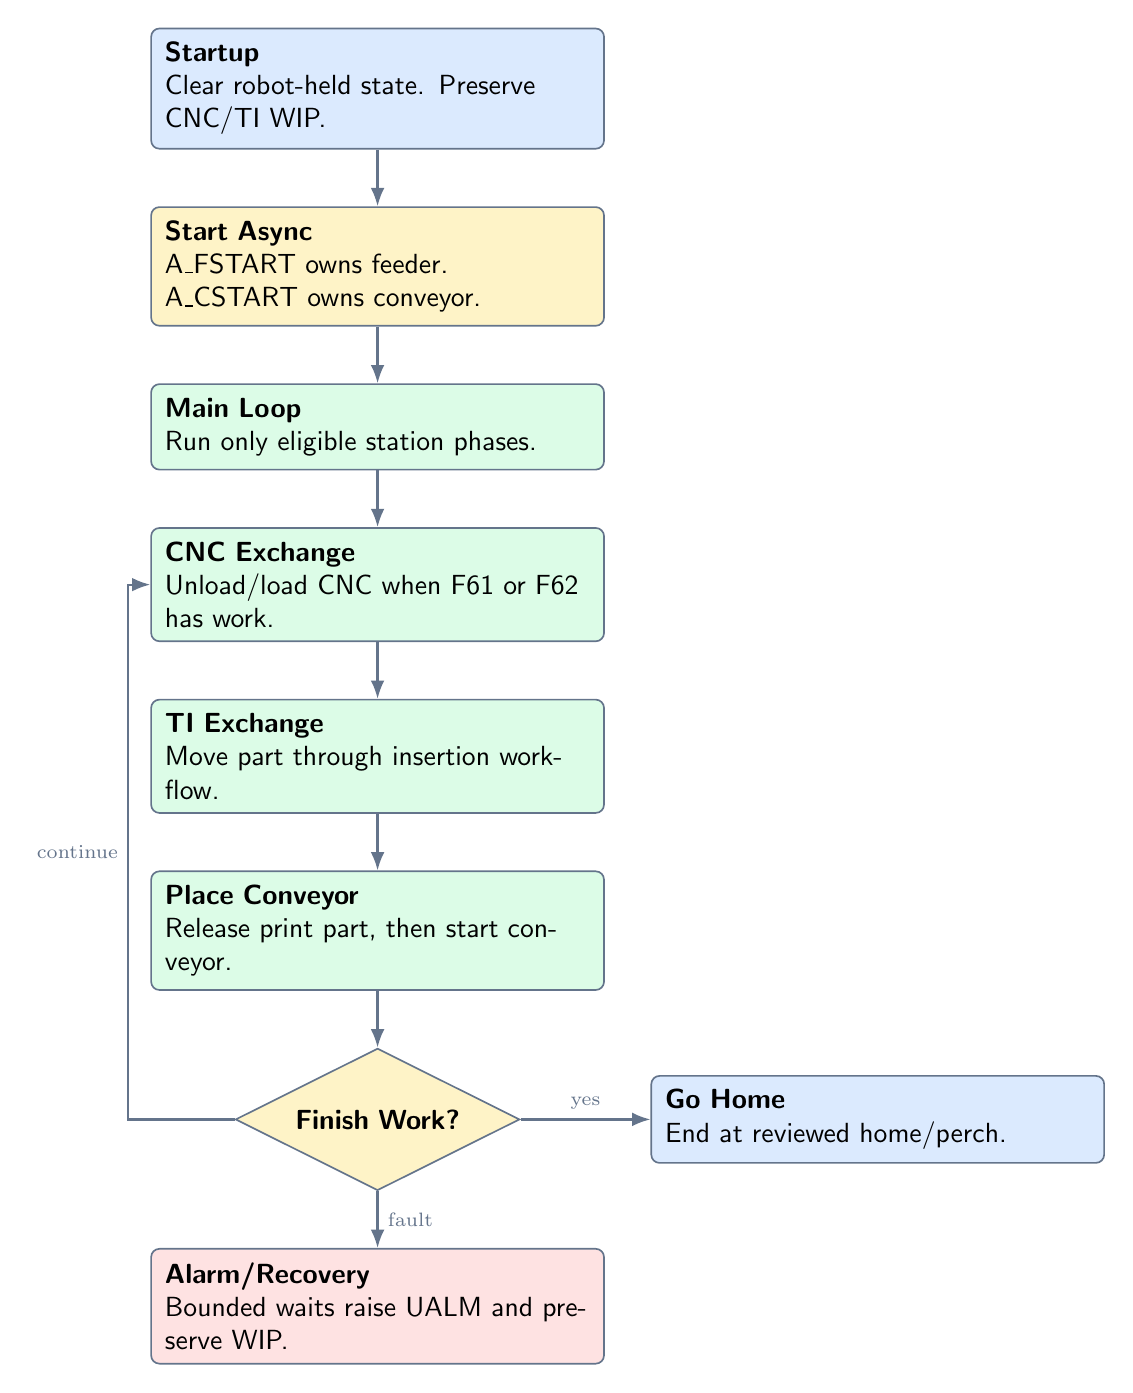
\begin{tikzpicture}[
  font=\sffamily,
  node distance=0.72cm and 1.65cm,
  flow/.style={
    rounded corners=3pt,
    draw=linegray,
    line width=0.6pt,
    align=left,
    text width=5.4cm,
    minimum height=1.0cm,
    inner sep=5pt
  },
  decision/.style={
    diamond,
    aspect=2.0,
    draw=linegray,
    line width=0.6pt,
    align=center,
    text width=2.7cm,
    inner sep=2pt
  },
  arrow/.style={-Latex, linegray, line width=0.8pt}
]

\node[flow, fill=nodeblue] (startup)
  {\textbf{Startup}\\Clear robot-held state. Preserve CNC/TI WIP.};
\node[flow, fill=nodeyellow, below=of startup] (async)
  {\textbf{Start Async}\\A\_FSTART owns feeder. A\_CSTART owns conveyor.};
\node[flow, fill=nodegreen, below=of async] (loop)
  {\textbf{Main Loop}\\Run only eligible station phases.};

\node[flow, fill=nodegreen, below=of loop] (cnc)
  {\textbf{CNC Exchange}\\Unload/load CNC when F61 or F62 has work.};
\node[flow, fill=nodegreen, below=of cnc] (ti)
  {\textbf{TI Exchange}\\Move part through insertion workflow.};
\node[flow, fill=nodegreen, below=of ti] (conv)
  {\textbf{Place Conveyor}\\Release print part, then start conveyor.};

\node[decision, fill=nodeyellow, below=of conv] (finish)
  {\textbf{Finish Work?}};
\node[flow, fill=nodeblue, right=of finish] (home)
  {\textbf{Go Home}\\End at reviewed home/perch.};
\node[flow, fill=nodered, below=of finish] (fault)
  {\textbf{Alarm/Recovery}\\Bounded waits raise UALM and preserve WIP.};

\draw[arrow] (startup) -- (async);
\draw[arrow] (async) -- (loop);
\draw[arrow] (loop) -- (cnc);
\draw[arrow] (cnc) -- (ti);
\draw[arrow] (ti) -- (conv);
\draw[arrow] (conv) -- (finish);
\draw[arrow] (finish) -- node[above, font=\scriptsize]{yes} (home);
\draw[arrow] (finish) -- node[right, font=\scriptsize]{fault} (fault);
\draw[arrow] (finish.west) -| ++(-1.35,0) |- node[pos=0.25, left, font=\scriptsize]{continue} (cnc.west);

\end{tikzpicture}
\end{document}
